\section{Dokumentation}
\label{backend-dokumentation}

Das Backend von \kort{} ist durchgängig mit der PHP-Dokumentationsprache \brand{PHPDoc}\footnote{\url{http://www.phpdoc.org/}} dokumentiert\footnote{Die Dokumentation findet sich unter: \url{http://kort.herokuapp.com/docs/Kort-backend}}.
Um sicherzustellen, dass die PHPDoc-Kommentare stets aktuell sind, haben wir deren Schema in unseren Code-Standard integriert.
Der Code-Standard wird automatisch überprüft und Abweichungen davon dem Benutzer angezeigt.
Die ganze Dokumentation wird jeweils beim builden neu generiert.

Grundsätzlich stellt die Dokumentation das öffentliche \gls{API} des Backends dar.
Alle privaten Funktionen sind aber ebenfalls dokumentiert, um einen einfachen Einstieg in die Weiterentwicklung der Applikation zu ermöglichen.

\begin{figure}[H]
	\centering
	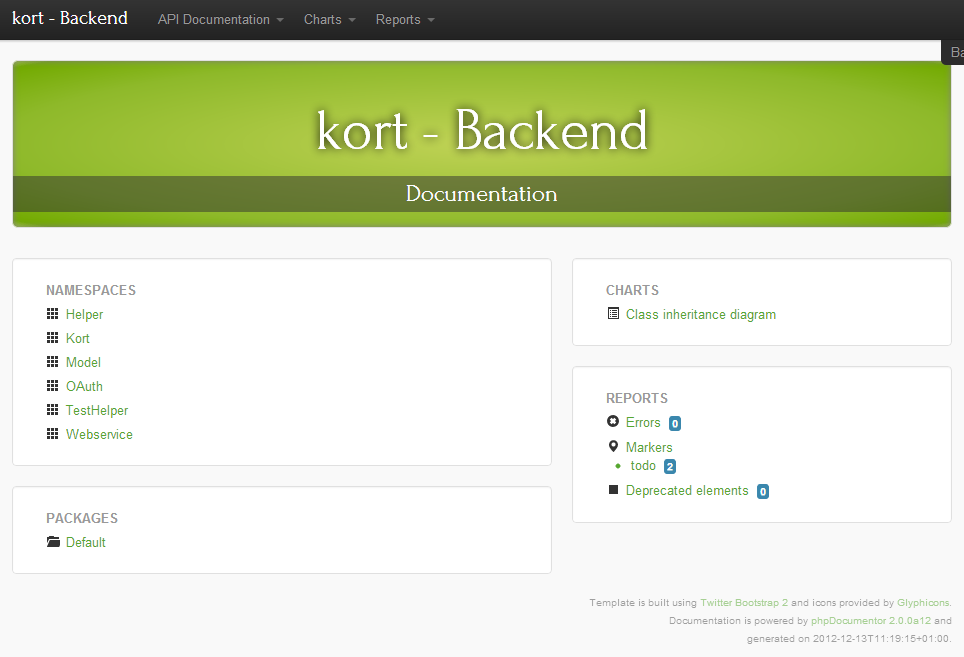
\includegraphics[width=\textwidth]{images/implementation/backend/kort-backend-documentation}
	\caption{\kort{} Backend Dokumentation mit PHPDoc}
	\label{image-kort-backend-documentation}
\end{figure}